\documentclass[border=6pt]{standalone}
\usepackage{amsmath,amssymb}
\usepackage{tikz}
\begin{document}
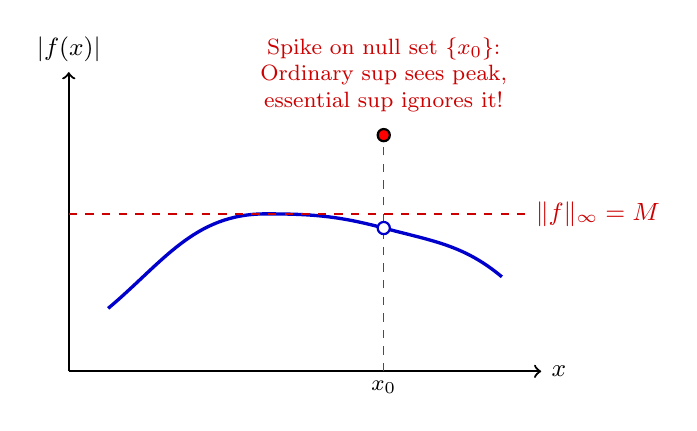
\begin{tikzpicture}[font=\small]
  \draw[->, thick] (0,0) -- (6.0,0) node[right] {$x$};
  \draw[->, thick] (0,0) -- (0,3.8) node[above] {$|f(x)|$};

  % Normal curve passing explicitly through (4.0, 1.82)
  \draw[very thick, blue!80!black]
    (0.5, 0.8) to[out=40, in=180] (2.5, 2.0) to[out=0, in=165] (4.0, 1.82) to[out=-15, in=140] (5.5, 1.2);

  % Essential supremum ceiling
  \draw[thick, dashed, red!80!black] (0, 2.0) -- (5.8, 2.0) node[right] {$\|f\|_\infty = M$};

  % Vertical dashed line and open circle on curve at x_0 = 4.0
  \draw[dashed, red] (4.0, 0) -- (4.0, 3.0);
  \node[below, font=\footnotesize] at (4.0, 0) {$x_0$};
  \draw[thick, blue!80!black, fill=white] (4.0, 1.82) circle (2.2pt);

  % Isolated spike on null set {x_0}
  \draw[thick, fill=red] (4.0, 3.0) circle (2.2pt);
  \node[font=\footnotesize, red!80!black, align=center, above=5pt] at (4.0, 3.0)
    {Spike on null set $\{x_0\}$:\\Ordinary sup sees peak,\\essential sup ignores it!};
\end{tikzpicture}
\end{document}
